\chapter{Présentation de l'entreprise}

\section{L'entreprise : Mimesis Republic}

Co-fondée par Nicolas Gaume et Sébastian Lombardo en 2007, Mimesis Republic est
une société française basée à Paris et Bordeaux, spécialisée dans les
technologies plurimedia (réseaux sociaux, web, jeux vidéo). Composée d’une
équipe de 47 personnes et d’un management expérimenté, à l’origine de nombreux
blockbusters dans le secteur de l’entertainment depuis plus de 15 ans, Mimesis
Republic a placé le projet Mamba Nation au cœur de sa stratégie à destination
des adolescents et des jeunes adultes. Mimesis Republic est financée par des
investisseurs privés issus du monde de l’entreprise.

\section{Le projet : Mamba Nation}

Mamba Nation est un univers dédié aux adolescents et jeunes adultes qui
ambitionne de relier la vie réelle et le monde virtuel avec les réseaux sociaux
comme passerelle.

Cet univers virtuel est accessible au sein d'un navigateur internet à travers
une applet Java. L'intégralité de son contenu est \textit{streamé}, aucun client n'est à
installer sur l'ordinateur de l'utilisateur.

Mamba Nation c’est le renouveau du réseau social qui se construit sur Facebook
en y amenant l’Avatar, les jeux, les outils, les marques dont les ados et les
jeunes adultes ont besoin.
La véritable innovation pour les jeunes comme pour les marques, ce n’est pas de
choisir entre le réel et le virtuel, c’est d’utiliser le virtuel pour positiver
et enrichir sa vie réelle. C’est ce que nous appelons l’EXTRA LIFE.

Dans Mamba Nation, Vous pouvez vous faire des amis, vous amuser ensemble, et
même obtenir de la reconnaissance à travers une multitude d’actions et
d’interactions. En résumé «  FRIENDS + FUN + FAME ».

Ici le jeu n’est pas une fin, c’est un moyen permettant à chacun de s’engager et
révéler sa véritable personnalité, son véritable caractère.
Chaque utilisateur peut donc créer son Avatar, voir ses différents avatars,
chatter, inviter des amis, draguer, danser et chanter, etc…

Mamba Nation est génératrice de moments forts (virtuels) et partagés
(réellement).

\subsection{Images de l'univers virtuel} 

\begin{figure}[H]
  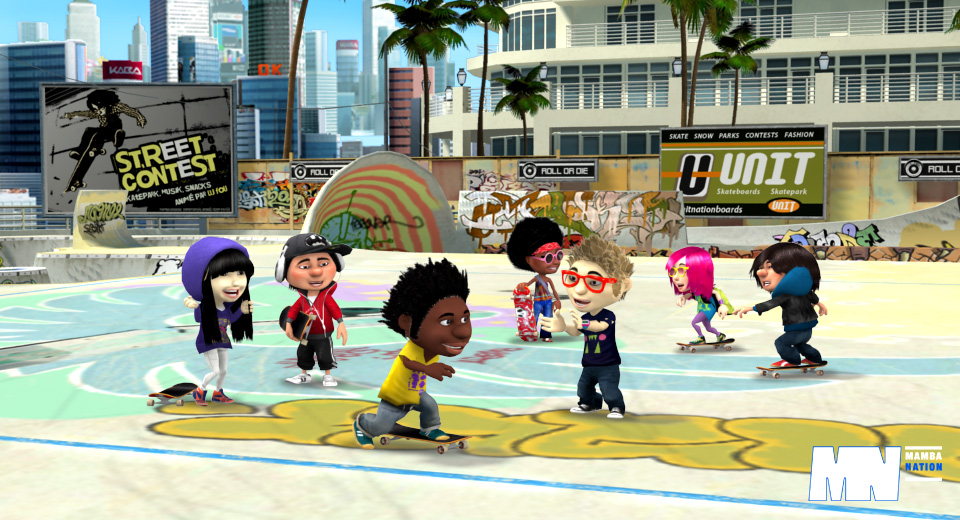
\includegraphics[width=\textwidth]{univers-skate.jpg}
  \caption{Tchater dans la Nation}
\end{figure}

\begin{figure}[H]
  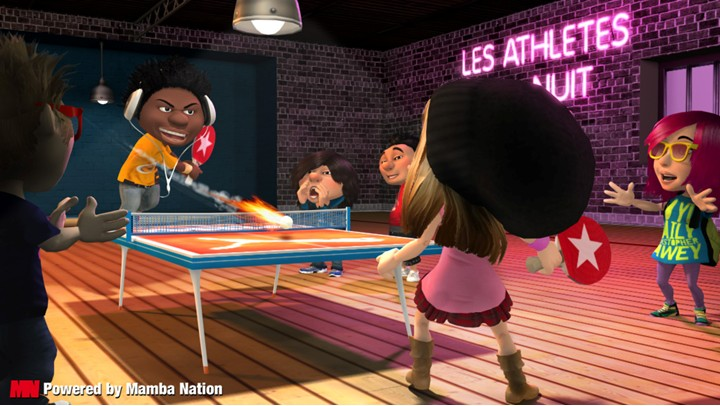
\includegraphics[width=\textwidth]{ping-pong.jpg}
  \caption{Une partie de ping pong dans la Nation}
\end{figure}

\begin{figure}[H]
  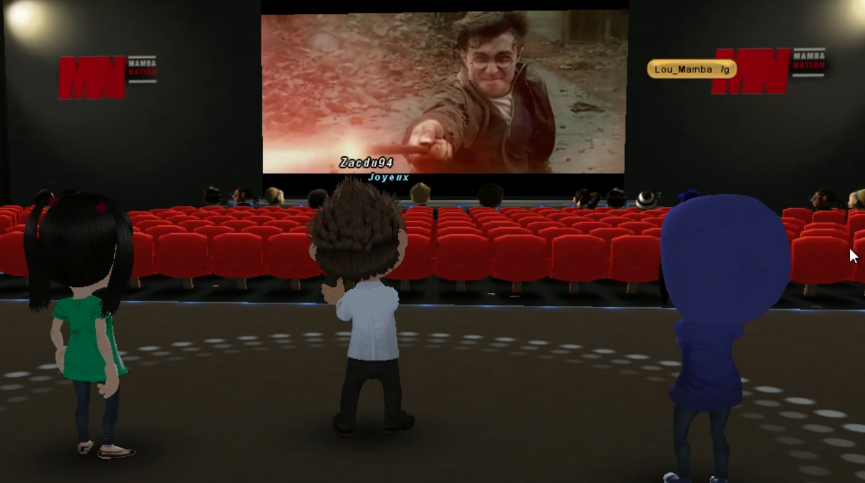
\includegraphics[width=\textwidth]{cinema.png}
  \caption{Regarder une vidéo Dailymotion en compagnie de ses potes}
\end{figure}

\section{Modèle économique}

La société mise sur un modèle Freemium, l'accès au service est gratuit, mais
pour obtenir ou utiliser certains biens virtuels tel que des vêtements ou des
animations d'avatar, les utilisateurs doivent acheter des "Blings" ou des
"Vibes", les monnaies virtuelles du site. La société vise un taux de 3 à 10\%
d'utilisateurs payant pour financer son service et être rentable sous 2 ans.

La société mise également sur la publicité et les évenements qu'elle organisera
dans ses salons 3D grâce à ces nombreux partenaires. Elle parle notamment de
concerts privées d'artiste avec leur avatar.

\section{Partenaires}

Mimesis Republic s'est entouré de partenaires importants pour développer son
produit notamment Xavier Niel, fondateur et vice-président du groupe Iliad, via
son fonds d’investissement Kima Ventures, Marc Simoncini, P-DG et fondateur du
site de rencontres Meetic, via son fonds d'investissement Jaina Capital, Steve
et Jean-Émile Rosenblum, fondateurs et dirigeants de Pixmania via leur fonds
d'investissement Dotcorp Asset Management, François Pinault, via sa holding
Artemis S.A, Laurent Schwarz co-fondateur d'Alten, Jean-François Cécillon ancien
président d'EMI France, Pascal Nègre P-DG de Universal Music France.

La société a annoncé qu'elle avait signé des partenariats pour enrichir son
univers virtuel avec :
\begin{itemize}
  \item[\textbullet]\textbf{Universal Music} pour promouvoir et lancer des artistes,
    réaliser des évènement musicaux, etc.
  \item[\textbullet]\textbf{Allociné} qui va animer des salons communautaires en
    3D autour de séries TV et de films
  \item[\textbullet]\textbf{Puma} qui va associer la Mamba Nation à ses
    campagnes publicitaires, et apporter des items virtuels
  \item[\textbullet]\textbf{Trace} qui va relooker l'habillage de ses chaînes de
    télévision (Trace TV, etc.) et de sa filiale de téléphonie mobile Trace
    Mobile
  \item[\textbullet]\textbf{DailyMotion} qui va streamer de la vidéo au sein de
    l’expérience
\end{itemize}

\section{Les équipes}
TODO
\subsection{L'équipe Architecture}

\subsection{L'équipe Engine}

\subsection{L'équipe Infrastructure}

\subsection{L'équipe Studio}

\subsection{L'équipe Expérience}

\begin{figure}[H]
  \begin{center}
    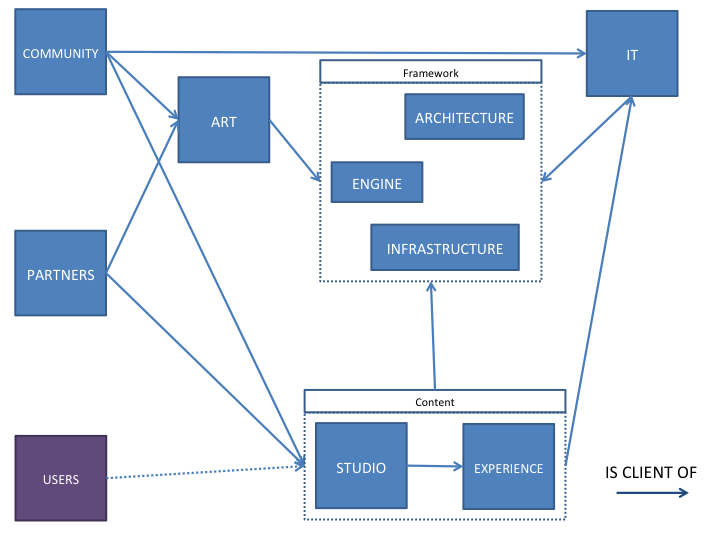
\includegraphics[width=\textwidth]{organisation.png}   
  \end{center}
  \caption{Les relations client/fournisseur}
\end{figure}

